\documentclass[10pt]{article}
\usepackage[T1]{fontenc}\usepackage[utf8]{inputenc}\usepackage{lmodern}
\usepackage[margin=18mm]{geometry}\usepackage{graphicx,hyperref,parskip}
\hypersetup{hidelinks}\setlength{\emergencystretch}{3em}
\begin{document}
\section*{Full-order twist seed: explicit failed candidate}
\textbf{Run:} generator-full-order-v1\par
The original candidate required a twist point whose order equals the whole rational twist group. The frozen native producer exits 1 with no full-order seed in fixed search; the output directory contains no complete RECORDS.json or GP script. One native execution was attempted, and the planned GP reference was unattempted. Do not report a completed 120-case census or infer missing costs as zero.

Source 9643e917\allowbreak{}922cca9c\allowbreak{}50ae9170\allowbreak{}9ba12f4e\allowbreak{}a9d6bfa1; protocol 248a8120\allowbreak{}237f48e6\allowbreak{}cd74022b\allowbreak{}f964582a\allowbreak{}898c876b\allowbreak{}c9b8ecc7\allowbreak{}3aed834f\allowbreak{}c031d8d2. Native cap600 seconds,4GiB,64MiB/file. The successor independently finds a noncyclic twist with structure C7 x C119; that group has no point of order833. The original rule remains unavailable there, rather than being silently changed.

The faithful actual-execution export passes standalone schema/file validation. Full protocol binding retains four findings for the absent GP execution. The initial planned-row export was also rejected because the schema forbids attempts=0; both records are retained. No reference execution is invented to make the checker green.

Raw archive 976 bytes, SHA256 998844ed\allowbreak{}b84d13ff\allowbreak{}70db937d\allowbreak{}6983215f\allowbreak{}f22f91b9\allowbreak{}e5b4bc74\allowbreak{}0489056b\allowbreak{}c93ef839; 3 file members verified after fresh download. The separate successor changes the rule for every fixture before its own data.

Local L0 managed Xeon Platinum 8573C/KVM, one native thread; no native time, calibrated field operations, GAE, fastest-external or full IC/rho result. The existing authorized local fallback follows the documented EKS access/image gap. Source, binaries, actual argv/env, exits, limits and input hashes are versioned; no paid resource or IAM change.

The inputs are all ten original public toy fixtures with registered source/twist identities. No target, shift, base size or observed yield enters seed selection. Final E28 labels 32–63 remain unopened. This is standard finite-group order/selection work, not a novelty or NIST-security result. Literature reviewed before design: predecessor reports/atlas, existing field/group source and local primary PARI ellorder/ellcard/ellgroup help.

Both raw archives use the user-confirmed Setec content-addressed store. Fresh downloads verify every member and identical deterministic repacking. Original failed data and the separately frozen successor remain distinct; no failed attempt is silently replaced.

\textbf{Sources:} {\footnotesize \path{execution-v6/PROTOCOL.md}; \path{execution-v6/FAILURE.json}; \path{execution-v6/experiment.export.json}; \path{execution-v6/RAW_VERIFICATION.json}}
\section*{Observed failure and unattempted reference}
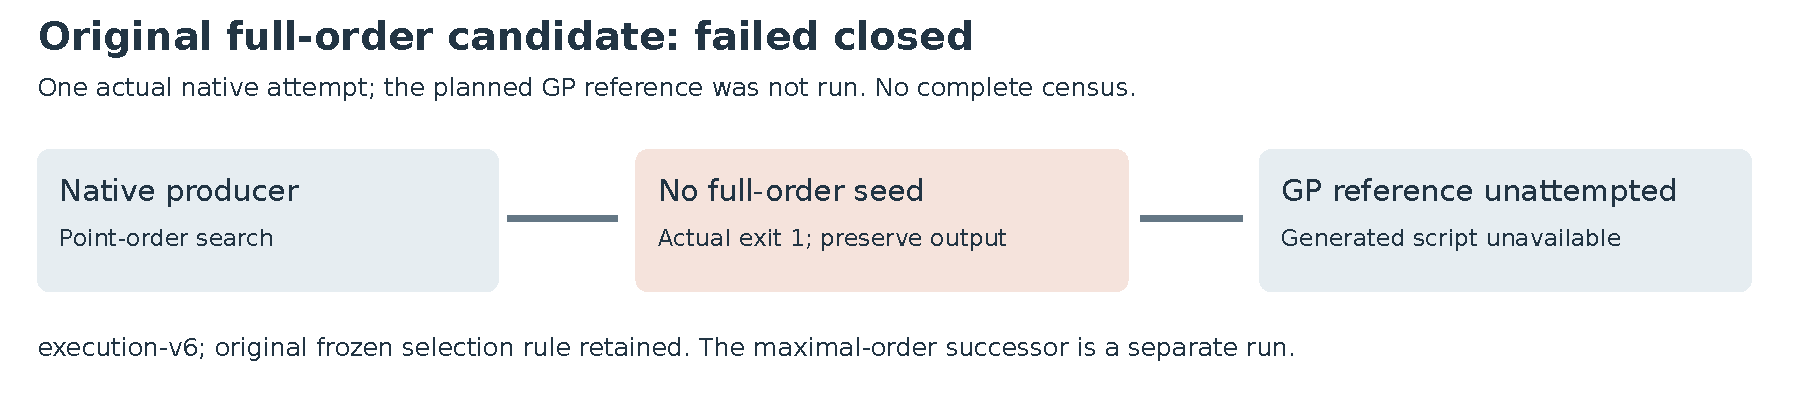
\includegraphics[width=\linewidth]{FLOW.pdf}
\end{document}
